\documentclass[12pt,a4paper]{article}

\usepackage{tikz} % Package for drawing
\usepackage{amsmath}
\usepackage{hyperref}
\usepackage{graphicx}
\usepackage{subcaption}
\usepackage{listings}
\usepackage{float}

%TITLE PAGE
\usepackage{float}
\usepackage[colorinlistoftodos]{todonotes}

\usepackage{fontspec}
\usepackage{xunicode}
\usepackage{xltxtra}
\usepackage{xgreek}
\setmainfont[Mapping=tex-text]{CMU Serif}
\title{Προσομοίωση βιολογικών νευρώνων σε συστήματα παράλληλης επεξεργασίας}
\author{Στρατής Τσιρτσής}
\date{11/11/2018}

\makeatletter
\let\anw@true\anw@false
\makeatother

\lstset{language=C,
                basicstyle=\ttfamily,
                keywordstyle=\color{blue}\ttfamily,
                breaklines=true,
                showstringspaces=false
}

\begin{document}

\begin{titlepage}

\newcommand{\HRule}{\rule{\linewidth}{0.5mm}} % Defines a new command for the horizontal lines, change thickness here

\center % Center everything on the page
 
%----------------------------------------------------------------------------------------
%	HEADING SECTIONS
%----------------------------------------------------------------------------------------

\begin{minipage}[t]{0.45\textwidth}
\centering
ΕΘΝΙΚΟ ΜΕΤΣΟΒΙΟ ΠΟΛΥΤΕΧΝΕΙΟ
\end{minipage}\hfill
\begin{minipage}[t]{0.45\textwidth}
\centering
ΕΘΝΙΚΟ ΚΕΝΤΡΟ ΕΡΕΥΝΑΣ ΦΥΣΙΚΩΝ ΕΠΙΣΤΗΜΩΝ ``ΔΗΜΟΚΡΙΤΟΣ''
\vspace{\baselineskip}
\end{minipage}

\begin{minipage}[t]{0.45\textwidth}
\centering

\includegraphics[width=0.5\textwidth]{Figures/ntua.jpg}
\end{minipage}\hfill
\begin{minipage}[t]{0.45\textwidth}
\centering
	
\includegraphics[width=0.5\textwidth]{Figures/dimokritos.jpg}
\end{minipage}

\begin{minipage}[t]{0.45\textwidth}
\centering
\vspace{\baselineskip}
Σχολή Ηλεκτρολόγων Μηχανικών \& Μηχανικών Υπολογιστών
\end{minipage}\hfill
\begin{minipage}[t]{0.45\textwidth}
\centering
\vspace{\baselineskip}
Ινστιτούτο Νανοεπιστήμης \& Νανοτεχνολογίας

\vspace{0.1cm}

Εργαστήριο Στατιστικής Μηχανικής \& Πολύπλοκων Δυναμικών Συστημάτων
\end{minipage}

\vspace{\baselineskip}
\vspace{\baselineskip}
\vspace{\baselineskip}
%----------------------------------------------------------------------------------------
%	TITLE SECTION
%----------------------------------------------------------------------------------------

\HRule \\[0.4cm]
{ \huge \bfseries Προσομοίωση βιολογικών νευρώνων σε συστήματα παράλληλης επεξεργασίας}\\[0.4cm] % Title of your document
\HRule \\[1.5cm]
 
%----------------------------------------------------------------------------------------
%	AUTHOR SECTION
%----------------------------------------------------------------------------------------

\begin{minipage}{0.4\textwidth}
\begin{flushleft} \large
\centering
Τσιρτσής Ευστράτιος % Your name
\end{flushleft}

\end{minipage}\\[2cm]

% If you don't want a supervisor, uncomment the two lines below and remove the section above
%\Large \emph{Author:}\\
%John \textsc{Smith}\\[3cm] % Your name

%----------------------------------------------------------------------------------------
%	DATE SECTION
%----------------------------------------------------------------------------------------

{\large \today}\\[2cm] % Date, change the \today to a set date if you want to be precise

\vfill % Fill the rest of the page with whitespace

\end{titlepage}

\newpage

\centerline{\noindent \textbf{Περίληψη}}
\vspace{0.5cm}
Το αντικείμενο της παρούσας πρακτικής άσκησης αφορά την προσομοίωση δικτύων βιολογικών νευρώνων κάνοντας χρήση τεχνικών παράλληλου προγραμματισμού. Συγκεκριμένα, εξετάζονται βελτιώσεις στον αλγόριθμο προσομοίωσης του μοντέλου Leaky Integrate-and-Fire σε Μη Τοπική Συνδεσιμότητα και στη συνέχεια γίνεται χρήση διαφόρων εργαλείων παραλληλισμού για την περαιτέρω επιτάχυνση της προσομοίωσης. Υλοποιείται παραλληλισμός νημάτων με χρήση των περιβαλλόντων προγραμματισμού PThreads και OpenMP και συγκρίνεται η χρονική βελτίωση που προσφέρουν ανάλογα με το διαθέσιμο αριθμό υπολογιστικών πόρων. Τέλος, γίνεται μία προσπάθεια παραλληλισμού σε κάρτα επεξεργασίας γραφικών με χρήση του εργαλείου CUDA και παρουσιάζονται συνολικά αποτελέσματα και συμπεράσματα για τις διάφορες μεθόδους που εξετάστηκαν. Η επιτάχυνση που παρατηρείται είναι αξιοσημείωτη, μειώνοντας το χρόνο της προσομοίωσης μέχρι και 10 φορές.

\newpage

\centerline{\noindent \textbf{Ευχαριστίες}}
\vspace{0.5cm}
Η παρούσα πρακτική άσκηση έγινε στο Εργαστήριο Στατιστικής Μηχανικής \& Πολύπλοκων Δυναμικών Συστημάτων του Ινστιτούτου Νανοεπιστήμης \& Νανοτεχνολογίας του ΕΚΕΦΕ ``Δημόκριτος'' στα πλαίσια του προγράμματος πρακτικής άσκησης της Σχολής Ηλεκτρολόγων Μηχανικών \& Μηχανικών Υπολογιστών του Εθνικού Μετσόβιου Πολυτεχνείου. Μέσα από αυτή είχα την ευκαιρία να συμμετέχω στο ερευνητικό περιβάλλον του ΕΚΕΦΕ ``Δημόκριτος'' και να γνωρίσω ενδιαφέροντες ανθρώπους. 

Αρχικά, θέλω να ευχαριστήσω την επιβλέπουσα Δρ. Αστέρω Προβατά που μου έδωσε την ευκαιρία να συμμετέχω στις δραστηριότητες του Εργαστηρίου και με καθοδήγησε σε όλα τα βήματά της πρακτικής άσκησης με τις χρήσιμες συμβουλές της. Επίσης, οφείλω ένα μεγάλο ευχαριστώ στην υπόλοιπη ομάδα του Εργαστηρίου, τη Νεφέλη Τσίγκρη, το Θοδωρή Κασιμάτη, τη Δέσποινα Γκατζιούρα, το Γιώργο Αργυρόπουλο, το Γιάννη Κουλιεράκη, το Γιώργο Καράκο, το Δημήτρη Θάνο και τον Παντελή Μελά, για τη συνεργασία τους και τις στιγμές που περάσαμε μαζί.

Ακόμα, θα ήθελα να ευχαριστήσω τον Επίκουρο Καθηγητή της Σχολής Ηλεκτρολόγων Μηχανικών \& Μηχανικών Υπολογιστών κ. Ιωάννη Γκόνο που ως ακαδημαϊκός υπεύθυνος του προγράμματος πρακτικής άσκησης της Σχολής, μου έδωσε τη δυνατότητα να συμμετάσχω σε αυτό και να αποκτήσω χρήσιμα εφόδια για την ακαδημαϊκή και επαγγελματική μου σταδιοδρομία.

Τέλος, θέλω να αναφέρω την προσφορά του Εθνικού Δικτύου Έρευνας και Τεχνολογίας για τη χρήση του υπερυπολογιστή Άρη (έργο pr005014), που χωρίς αυτόν δεν θα ήταν δυνατή η παραγωγή μέρους των αποτελεσμάτων της παρούσας εργασίας.

\newpage

\tableofcontents
\newpage
\listoffigures
\newpage

\section{Εισαγωγή}

\subsection{Το Φυσικό Πρόβλημα}

Τα τελευταία χρόνια, ένα πεδίο έρευνας που έχει συγκεντρώσει μεγάλο ενδιαφέρον της παγκόσμιας επιστημονικής κοινότητας είναι αυτό της νευροεπιστήμης, δηλαδή της κατανόησης της δομής και λειτουργίας του εγκεφάλου. Πρόκειται για ένα πολυσυλλεκτικό ερευνητικό τομέα με τον οποίο ασχολούνται άνθρωποι με γνώσεις ιατρικής, βιολογίας, φυσικής, χημείας, μαθηματικών και πληροφορικής προκειμένου να κατανοήσουν τα πολύπλοκα φαινόμενα του εγκεφάλου και να λύσουν το ``γρίφο'' της ανθρώπινης νοημοσύνης και τα προβλήματα των νευροεκφυλιστικών νόσων.

Η μελέτη της δυναμικής συμπεριφοράς πολύπλοκων συστημάτων και ιδιαίτερα η συλλογική συμπεριφορά που αναπτύσσεται από τη σύζευξη ταλαντωτών παρουσιάζει ιδιαίτερο ενδιαφέρον. Μάλιστα, ο \textit{συγχρονισμός} συζευγμένων ταλαντωτών αποτελεί χαρακτηριστικό φαινόμενο αυτο-οργάνωσης της ύλης και κατέχει εξέχουσα θέση στη μελέτη συστημάτων που αποτελούνται από μεγάλο πλήθος αλληλεπιδρώντων στοιχείων. Ένα τέτοιο σύστημα αποτελεί και το δίκτυο των νευρώνων του εγκεφάλου για το οποίο υπάρχει πλήθος μελετών στο ευρύτερο πεδίο της υπολογιστικής νευροεπιστήμης και ιδιαίτερα ως προς την ανάπτυξη φαινομένων συγχρονισμού.

Ένα φαινόμενο συγχρονισμού, το οποίο έχει προκαλέσει ιδιαίτερο επιστημονικό ενδιαφέρον και το οποίο απαντάται και στην περίπτωση δικτύων που χαρακτηρίζονται από δυναμική μοντέλων νευρώνων, είναι η \textit{χιμαιρική κατάσταση}. Η χιμαιρική κατάσταση χαρακτηρίζεται από τη συνύπαρξη συγχρονισμένων και ασυγχρόνιστων περιοχών σε συστήματα όμοιων ταλαντωτών. Το όνομα χιμαιρική κατάσταση προέρχεται από τη Χίμαιρα, πλάσμα της αρχαίας ελληνικής μυθολογίας το οποίο είχε 3 κεφάλια, λιονταριού, κατσίκας και φιδιού. Οι πρώτοι που μελέτησαν το φαινόμενο των χιμαιρικών καταστάσεων σε συστήματα συνδεδεμένων ταλαντωτών ήταν οι Kuramoto και Battogtokh \cite{kuramoto_coexistence_2002}, ενώ στη συνέχεια οι χιμαιρικές καταστάσεις εντοπίστηκαν και μελετήθηκαν για πληθώρα δυναμικών συστημάτων όπως νευρωνικά \cite{hizanidis_chimera_2014}, μηχανικά \cite{martens_chimera_2013} και χημικά \cite{tinsley_chimera_2012} συστήματα.

Ο σκοπός της παρούσας εργασίας είναι η χρήση τεχνικών παράλληλου προγραμματισμού προκειμένου να γίνει αποδοτικά η προσομοίωση τέτοιων πολύπλοκων συστημάτων και ο εντοπισμός χιμαιρικών καταστάσεων. Στη συνέχεια αυτού του κεφαλαίου, παρουσιάζεται η απαραίτητη θεωρία γύρω από το φυσικό πρόβλημα και η αναγκαιότητα της εργασίας αυτής. Στο Κεφάλαιο 2, αναλύονται οι τεχνικές παράλληλου προγραμματισμού που χρησιμοποιήθηκαν, οι διαφορές τους και τα αντίστοιχα πλεονεκτήματα/μειονεκτήματα αυτών. Στο Κεφάλαιο 3, γίνεται αναλυτική παρουσίαση των σημείων ενδιαφέροντος του κώδικα προσομοίωσης. Στο Κεφάλαιο 4, παρατίθενται συγκριτικά αποτελέσματα των διαφόρων τεχνικών. Τέλος, στο Κεφάλαιο 5, γίνεται σχολιασμός των αποτελεσμάτων, αναφέρονται τα προβλήματα που εντοπίστηκαν και παρουσιάζονται τα τελικά συμπεράσματα της εργασίας.

\subsection{Στοιχεία Θεωρίας}

Οι τεχνικές παραλληλοποίησης που θα αναλυθούν στη συνέχεια, είναι ανεξάρτητες των λεπτομερειών του μοντέλου που προσομοιώνεται και μπορούν να εφαρμοστούν για τη μελέτη οποιουδήποτε προβλήματος παρόμοιας φύσης. Παρ' όλα αυτά, λόγω ύπαρξης προηγούμενων αποτελεσμάτων \cite{schmidt_chimera_2017}, για την αξιολόγηση των πειραμάτων χρησιμοποιήθηκε το μοντέλο Leaky Integrate-and-Fire για τη λειτουργία του κάθε νευρώνα και Μη-Τοπική Συνδεσιμότητα (Non-Local Connectivity) σε 2 διαστάσεις για τη μορφή του δικτύου.

Το μοντέλο \textbf{Leaky Integrate-and-Fire} περιγράφει τη χρονική μεταβολή του δυναμικού μεμβράνης ενός νευρώνα. Η βασική διαφορική εξίσωση ενός μεμονωμένου νευρώνα σύμφωνα με το μοντέλο είναι η εξής:

\begin{equation}
\frac{du(t)}{dt} = \mu - u(t)
\end{equation}

Η μεταβλητή $u$ αντιστοιχεί στο δυναμικό μεμβράνης ενός νευρώνα, ενώ η σταθερά $\mu$ είναι ένα άνω όριο του οποίου την τιμή το δυναμικό τείνει να προσεγγίσει. Πειραματικά, έχει παρατηρηθεί ότι το δυναμικό των νευρώνων αυξάνεται μέχρι να φτάσει κάποιο κατώφλι (αποπόλωση) και αμέσως μετά επανέρχεται ακαριαία στην κατάσταση ηρεμίας (επαναπόλωση). Για να προστεθεί αυτή η συμπεριφορά, το μοντέλο Leaky Integrate-and-Fire έχει την επιπλέον παρακάτω ιδιότητα:

\begin{equation}
\lim_{\varepsilon \to 0} u(t+\varepsilon)=0 ,u \geq u_{th}
\end{equation}

Η χρονική συμπεριφορά του δυναμικού ενός νευρώνα που ακολουθεί το μοντέλο αυτό φαίνεται στο Σχήμα 1.α.
 
\begin{figure}[h!]
  \centering
  \begin{subfigure}[b]{0.45\linewidth}
    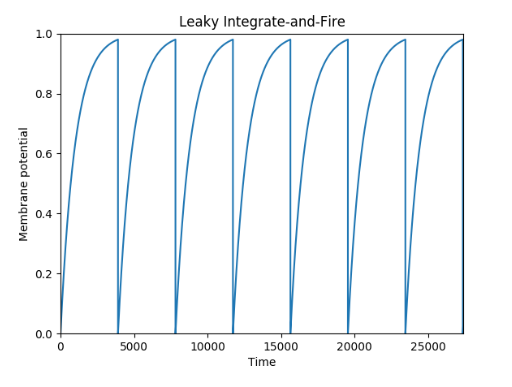
\includegraphics[width=\linewidth]{Figures/osc.png}
    \caption{Χωρίς περίοδο εφησυχασμού}
  \end{subfigure}
  \begin{subfigure}[b]{0.45\linewidth}
    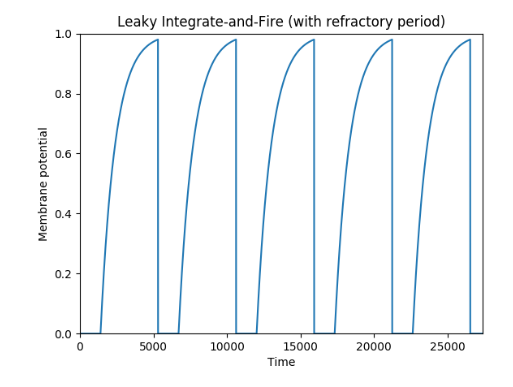
\includegraphics[width=\linewidth]{Figures/osc_refrac.png}
    \caption{Με περίοδο εφησυχασμού $0.35T_s$}
  \end{subfigure}
  \caption{Χρονική εξέλιξη του δυναμικού μεμβράνης ενός LIF ταλαντωτή}
\end{figure}

Μία ακόμα ιδιότητα που προέρχεται από παρατηρήσεις βιολογικών νευρώνων είναι η αδυναμία τους να αποπολωθούν κατά τη διάρκεια ενός μικρού χρονικού διαστήματος μετά την επαναπόλωσή τους. Το διάστημα αυτό αποκαλείται \textbf{Περίοδος Εφησυχασμού} $p_r$ (Refractory Period). Η διαφοροποίηση στη συμπεριφορά ενός νευρώνα με την προσθήκη αυτής της ιδιότητας φαίνεται στο Σχήμα 1.β.

Για τη δημιουργία του δικτύου χρησιμοποιείται τοπολογία \textbf{Μη-Τοπικής Συνδεσιμότητας }(Non-Local Connectivity) με τοροειδείς οριακές συνθήκες. Οι νευρώνες είναι διατεταγμένοι σε ένα δισδιάστατο πλέγμα μεγέθους $N \times N$ και ο κάθε νευρώνας $(i,j)$ είναι συνδεδεμένος, όχι μόνο με τους γειτονικούς του, αλλά και με όλους τους νευρώνες που ανήκουν στο τετράγωνο πλευράς $2R+1$ με κέντρο τον $(i,j)$. Σχετικά με τις οριακές συνθήκες, θεωρούμε ότι, αν το τετράγωνο υπερβεί τα όρια του πλέγματος, συνεχίζει στην ``απέναντι'' πλευρά. Η τοπολογία αυτή εκφράζεται αυστηρά (αγνοώντας τις οριακές συνθήκες) με τον παρακάτω τύπο:

\begin{equation}
\begin{split}
N_{ij} = \{(k,l) \in {[1,N]}^{2} \ | \ i-R \leq k \leq i+R 
\ \wedge \ j-R \leq l \leq j+R \} \\
\forall (i,j) \in {[1,N]}^{2} \ ,[1,N] = \{1,2,...,N\}
\end{split}
\end{equation}

Στο Σχήμα 2 απεικονίζονται διαισθητικά με πράσινο χρώμα ο νευρώνας $(i,j)$ ενώ με κόκκινο χρώμα η γειτονικοί του νευρώνες $N_{ij}$.
 
\begin{figure}[h!]
\centering
\begin{subfigure}[b]{0.45\linewidth}
	\begin{tikzpicture}[scale=0.85]
	\foreach \x in {0,...,6}{ 
		\foreach \y in {0,...,6}{
			\if \x 4
				\if \y 4
					\draw[fill=black!20!green] (\x,\y) circle (0.3);		
				\else
					\draw (\x,\y) circle (0.3);
				\fi		
			\else
				\draw (\x,\y) circle (0.3);
			\fi  
		}
	}
	\draw[fill=red, fill opacity = 0.3] (6.5,6.5) rectangle (1.5,1.5);
	\draw[<->] (4,6.8) -- node[,above] {R=2} (6,6.8);		
	\end{tikzpicture}
    \caption{Γειτονικοί νευρώνες}
\end{subfigure}
\begin{subfigure}[b]{0.45\linewidth}
	\begin{tikzpicture}[scale=0.85]
	\foreach \x in {0,...,6}{ 
		\foreach \y in {0,...,6}{
			\if \x 5
				\if \y 5
					\draw[fill=black!20!green] (\x,\y) circle (0.3);		
				\else
					\draw (\x,\y) circle (0.3);
				\fi		
			\else
				\draw (\x,\y) circle (0.3);
			\fi  
		}
	}
	\draw[draw=none, fill=red, fill opacity = 0.3] (6.5,6.5) rectangle (2.5,2.5);
	\draw[draw=none, fill=red, fill opacity = 0.3] (2.5,-0.5) rectangle (6.5,0.5);
	\draw[draw=none, fill=red, fill opacity = 0.3] (-0.5,-0.5) rectangle (0.5,0.5);
	\draw[draw=none, fill=red, fill opacity = 0.3] (-0.5,2.5) rectangle (0.5,6.5);
	\draw (-0.5,0.5) -- (0.5,0.5);
	\draw (0.5,0.5) -- (0.5,-0.5);
	\draw (2.5,-0.5) -- (2.5,0.5);
	\draw (2.5,0.5) -- (6.5,0.5);
	\draw (2.5,6.5) -- (2.5,2.5);
	\draw (2.5,2.5) -- (6.5,2.5);
	\draw (-0.5,2.5) -- (0.5,2.5);
	\draw (0.5,2.5) -- (0.5,6.5);	
	\draw[<->] (3,6.8) -- node[,above] {R=2} (5,6.8);		
	\end{tikzpicture}
    \caption{Τοροειδείς οριακές συνθήκες}
\end{subfigure}
\caption{Παράσταση Μη-Τοπικής Συνδεσιμότητας σε 2D}
\end{figure}

Προκειμένου να λάβουμε υπόψιν την αλληλεπίδραση του κάθε νευρώνα με τους γειτονικούς του, προσθέτουμε στη διαφορική εξίσωση του δυναμικού και έναν όρο που είναι ανάλογος της μέσης διαφοράς του δυναμικού του νευρώνα $(i,j)$ με τους υπόλοιπους στο σύνολο $N_{ij}$. Η διαφορική εξίσωση διαμορφώνεται ως εξής:
\hypertarget{difeq}{
\begin{equation}
\frac{du_{ij}(t)}{dt} = \mu - u_{ij}(t) + \frac{\sigma}{\mid N_{ij} \mid -1}\sum_{(k,l) \in N_{ij}}^{}(u_{ij}(t)-u_{kl}(t)) \ ,\forall (i,j) \in {[1,N]}^{2}
\end{equation}
}

\noindent όπου $\sigma$ είναι ο συντελεστής σύζευξης (coupling strength) και δηλώνει το πόσο ενεργό ρόλο έχει στη διαμόρφωση του δυναμικού του νευρώνα η αλληλεπίδραση με τους γειτονικούς του.

\subsection{Προβλήματα στην πράξη}

Η μελέτη τέτοιων δικτύων νευρώνων που αντιστοιχούν σε πραγματικούς εγκεφάλους ανθρώπων είναι μία δυσκολότερη υπόθεση. Αυτό συμβαίνει διότι είναι πάρα πολύ δύσκολο να βρεθούν δεδομένα προερχόμενα από πραγματικούς ανθρώπους που να αφορούν την τοπολογία των νευρώνων τους σε τόσο μικροσκοπικό επίπεδο. Επιπλέον, λόγω του ότι σε πραγματικά δεδομένα η συνδεσιμότητα των νευρώνων περιέχει πολύπλοκα μοτίβα, για να απεικονιστεί αυτή η πολύπλοκη δομή σε υπολογιστικά συστήματα, το μέγεθος μνήμης που θα χρειαζόταν θα ήταν υπερβολικά μεγάλο.

Επίσης, ο ανθρώπινος εγκέφαλος περιέχει κατά μέσο όρο γύρω στα 16 δισεκατομμύρια νευρώνες που ο καθένας έχει γύρω στις 7000 συνδέσεις. Όπως είναι φυσικό, η προσομοίωση ενός συστήματος τόσο μεγάλου μεγέθους σε υπολογιστή θα απαιτούσε τεράστιο χρόνο ή αριθμό υπολογιστικών πόρων που είναι ανύπαρκτος την παρούσα στιγμή.

Για τους παραπάνω λόγους, οι μελέτες τέτοιων φαινομένων, περιορίζονται σε πιο απλές γενικευμένες τοπολογίες και σε σχετικά μικρό αριθμό νευρώνων προκειμένου να μπορούν να εξαχθούν γρήγορα και χρήσιμα συμπεράσματα. Για τις ανάγκες μελέτης πολυπλοκότερων μοντέλων και μεγαλύτερων συστημάτων, εξελιγμένες υπολογιστικές τεχνικές όπως αυτή της παραλληλοποίησης κρίνονται πλήρως αναγκαίες.

\newpage

\section{Τεχνικές Παράλληλου Προγραμματισμού}

\subsection{Μοντέλα Παραλληλισμού}
Εδώ και πολλά χρόνια, ως πρόγραμμα ορίζεται μία ακολουθία εντολών που οδηγούνται προς εκτέλεση στην κεντρική μονάδα επεξεργασίας ενός υπολογιστή. Οι εντολές αυτές εκτελούνται η μία μετά την άλλη ακολουθώντας μια λογική σειρά. Αυτό αποκαλείται \textit{σειριακό μοντέλο εκτέλεσης} και ένα παράδειγμα φαίνεται στο Σχήμα 3. Το πρόγραμμά του Σχήματος 3, υπολογίζει το χρώμα δύο τετραγώνων με βάση κάποιο κριτήριο.

\begin{figure}[h!]
	\centering
	\begin{tikzpicture}[scale=1]
	\draw (2,10) node[fill=blue!40, draw, rounded corners](par1) {Αρχή};
	\draw (2,8.5) node[fill=blue!40, draw, rounded corners, align=center](par2) {Υπολογισμός \\ δεξιού χρώματος};
	\draw (2,7) node[fill=blue!40, draw, rounded corners, align=center](par3) {Υπολογισμός \\ αριστερού χρώματος};
	\draw (par1) -- (par2);
	\draw (par2) -- (par3);
	\draw (0.5,9.75) rectangle (0.75,10);
	\draw (0.75,9.75) rectangle (1,10);
	\draw (-0.25,8) rectangle (0,8.25);
	\draw[fill=red] (0,8) rectangle (0.25,8.25);	
	\draw[fill=green] (-0.75,6.5) rectangle (-0.5,6.75);
	\draw[fill=red] (-0.5,6.5) rectangle (-0.25,6.75);
	\end{tikzpicture}
	\caption{Παράσταση σειριακού μοντέλου εκτέλεσης}
\end{figure}

Παρ' όλα αυτά, τα τελευταία περίπου 20 χρόνια, οι εξελίξεις στην σχεδίαση του hardware έχουν δώσει τη δυνατότητα κατασκευής πολυπύρηνων επεξεργαστών, δηλαδή επεξεργαστών που μπορούν να εκτελούν πάνω από μία εντολή ταυτόχρονα.

Αυτή η νέα δυνατότητα, οδήγησε στην ταχεία ανάπτυξη του Παράλληλου Προγραμματισμού \cite{noauthor_parallel_2018}, δηλαδή ενός συνόλου εργαλείων και τεχνικών που εκμεταλλεύονται τις ιδιότητες του υλικού προκειμένου να υλοποιήσουν μεγάλο αριθμό υπολογισμών σε πολύ μικρότερο χρόνο από ό,τι προηγουμένως. Αυτό γίνεται διατηρώντας ένα μέρος του προγράμματος σε σειριακή μορφή και μοιράζοντας ένα άλλο μέρος (συνήθως με βαρείς υπολογισμούς) στους διαθέσιμους πυρήνες του επεξεργαστή. Τα δύο βασικά μοντέλα παραλληλισμού είναι α)το \textit{επίπεδο διεργασιών} (process-level parallelism) και β)το \textit{επίπεδο νημάτων} (thread-level parallelism).

Στον παραλληλισμό διεργασιών, η ροή του προγράμματος αρχικά ελέγχεται από ένα πρόγραμμα-γονέα που δημιουργεί ανεξάρτητα προγράμματα-παιδιά καθένα από τα οποία αναλαμβάνει κάποια συγκεκριμένη εργασία. Μόλις η εργασία τους ολοκληρωθεί, η λειτουργία τους τερματίζεται και απομένει μόνο το πρόγραμμα-γονέας. Η επικοινωνία μεταξύ ``γονέα'' και ``παιδιών'' γίνεται αποκλειστικά με ειδικούς μηχανισμούς ανταλλαγής μηνυμάτων. Κατά τη δημιουργία τους, τα προγράμματα-παιδιά κληρονομούν ένα αντίγραφο της μνήμης (RAM) του προγράμματος-γονέα αλλά στη συνέχεια το τμήμα της μνήμης που διαχειρίζεται το κάθε πρόγραμμα από τα παραπάνω είναι διαφορετικό. Παρακάτω παρουσιάζεται σε διάγραμμα το πρόγραμμα του προηγούμενου παραδείγματος, παραλληλοποιημένο σύμφωνα με το μοντέλο παραλληλισμού διεργασιών.

\begin{figure}[h!]
	\centering
	\begin{tikzpicture}[scale=1]
	\draw (2,10) node[fill=blue!40, draw, rounded corners](par1) {Γονέας};
	\draw (2,4) node[fill=blue!40, draw, rounded corners](par2) {Παραλαβή};
	\draw (6,9) node[fill=blue!40, draw, rounded corners](son1) {Παιδί 1};
	\draw (6,7.5) node[fill=blue!40, draw, rounded corners, align=center](son2) {Υπολογισμός \\ δεξιού χρώματος};
	\draw (6,6) node[fill=blue!40, draw, rounded corners](son3) {Αποστολή};
	\draw (11,9) node[fill=blue!40, draw, rounded corners](dau1) {Παιδί 2};
	\draw (11,7.5) node[fill=blue!40, draw, rounded corners, align=center](dau2) {Υπολογισμός \\ αριστερού χρώματος};
	\draw (11,6) node[fill=blue!40, draw, rounded corners](dau3) {Αποστολή};
	\draw (par1) -- (par2);
	\draw[dotted] (par1) -- (son1);
	\draw[dotted] (par1) -- (dau1);
	\draw (son1) -- (son2);
	\draw (son2) -- (son3);
	\draw (dau1) -- (dau2);
	\draw (dau2) -- (dau3);
	\draw[dotted] (son3) .. controls +(down:2cm) and +(right:1cm) .. node[above,sloped] {Κόκκινο} (par2);
	\draw[dotted] (dau3) .. controls +(down:2cm) and +(right:1cm) .. node[above,sloped] {Πράσινο} (par2);
	\draw (0.5,9.75) rectangle (0.75,10);
	\draw (0.75,9.75) rectangle (1,10);
	\draw (4.5,8.75) rectangle (4.75,9);
	\draw (4.75,8.75) rectangle (5,9);
	\draw (9.5,8.75) rectangle (9.75,9);
	\draw (9.75,8.75) rectangle (10,9);
	\draw (3.5,7) rectangle (3.75,7.25);
	\draw[fill=red] (3.75,7) rectangle (4,7.25);
	\draw[fill=green] (8.25,7) rectangle (8.5,7.25);
	\draw (8.5,7) rectangle (8.75,7.25);
	\draw[fill=green] (0.25,3.75) rectangle (0.5,4);
	\draw[fill=red] (0.5,3.75) rectangle (0.75,4);
	\end{tikzpicture}
	\caption{Παράσταση αλγορίθμου με παραλληλισμό επιπέδου διεργασιών}
\end{figure}

Στην περίπτωση του παραλληλισμού νημάτων, η ροή του προγράμματος ελέγχεται όμοια, αρχικά από ένα πρόγραμμα-γονέα που δημιουργεί προγράμματα-παιδιά τα οποία αναλαμβάνουν να εκτελέσουν κάποια εργασία. Η κύρια διαφορά με τον παραλληλισμό διεργασιών είναι ότι τα προγράμματα-παιδιά δεν κληρονομούν ένα αντίγραφο της μνήμης (RAM) του προγράμματος-γονέα, αλλά έχουν τη δυνατότητα να γράφουν απευθείας πάνω στο αρχικό τμήμα μνήμης. Στο Σχήμα 5, παρουσιάζεται σε διάγραμμα το πρόγραμμα του Σχήματος 4, παραλληλοποιημένο σύμφωνα με το μοντέλο παραλληλισμού νημάτων.

Για την προσομοίωση του μοντέλου LIF με Μη-Τοπική Συνδεσιμότητα, είναι σημαντικό να παρατηρηθεί ότι η πραγματοποίηση του υπολογισμού του δυναμικού για ένα και μόνο στοιχείο του πλέγματος, όπως περιγράφεται στο Κεφάλαιο 1, απαιτεί τη γνώση του δυναμικού όλων των υπολοίπων στοιχείων σε ένα τετράγωνο πλευράς 2R+1. Ακόμα και για μικρές τιμές του R, ο αριθμός αυτών των στοιχείων είναι πολύ μεγάλος. Π.χ. για $R=10$ ο αριθμός των γειτονικών νευρώνων γίνεται $(2R+1)^{2}-1=440$. Συνεπώς, σε περίπτωση παραλληλισμού, το κάθε πρόγραμμα παιδί θα πρέπει να γνωρίζει ένα μεγάλο αριθμό τιμών που προέρχονται από υπολογισμούς άλλων προγραμμάτων-παιδιών. Στον παραλληλισμό επιπέδου διεργασιών, αυτό θα απαιτούσε αλληλοεξάρτηση και συνεχή επικοινωνία των προγραμμάτων-παιδιών προσθέτοντας μεγάλη καθυστέρηση στην εκτέλεση του προγράμματος. Γι' αυτό το λόγο, το ιδανικό μοντέλο για προσομοιώσεις τέτοιου τύπου είναι του παραλληλισμού επιπέδου νημάτων, όπου η πρόσβαση σε κοινή μνήμη δεν δημιουργεί την ανάγκη επιπλέον επικοινωνίας.

\begin{figure}[h!]
	\centering
	\begin{tikzpicture}[scale=1]
	\draw (2,10) node[fill=blue!40, draw, rounded corners](par1) {Γονέας};
	\draw (2,4.5) node[fill=blue!40, draw, rounded corners](par2) {Join};
	\draw (6,9) node[fill=blue!40, draw, rounded corners](son1) {Παιδί 1};
	\draw (6,6.5) node[fill=blue!40, draw, rounded corners, align=center](son2) {Υπολογισμός \\ δεξιού χρώματος};
	\draw (11,9) node[fill=blue!40, draw, rounded corners](dau1) {Παιδί 2};
	\draw (11,7.5) node[fill=blue!40, draw, rounded corners, align=center](dau2) {Υπολογισμός \\ αριστερού χρώματος};
	\draw (par1) -- (par2);
	\draw[dotted] (par1) -- (son1);
	\draw[dotted] (par1) -- (dau1);
	\draw (son1) -- (son2);
	\draw (dau1) -- (dau2);
	\draw[dotted] (son2) .. controls +(down:1.5cm) and +(right:1cm) .. node[above,sloped] {} (par2);
	\draw[dotted] (dau2) .. controls +(down:2cm) and +(right:1cm) .. node[above,sloped] {} (par2);
	\draw (0.5,9.75) rectangle (0.75,10);
	\draw (0.75,9.75) rectangle (1,10);
	\draw[fill=green] (0.5,7.25) rectangle (0.75,7.5);
	\draw (0.75,7.25) rectangle (1,7.5);
	\draw[fill=green] (0.5,6.25) rectangle (0.75,6.5);
	\draw[fill=red] (0.75,6.25) rectangle (1,6.5);
	\draw[fill=green] (0.5,4.25) rectangle (0.75,4.5);
	\draw[fill=red] (0.75,4.25) rectangle (1,4.5);
	\end{tikzpicture}
	\caption{Παράσταση αλγορίθμου με παραλληλισμό επιπέδου νημάτων}
\end{figure}

\subsection{Posix Threads}

Τα POSIX Threads (PThreads) \cite{noauthor_posix_2018} αποτελούν ένα προγραμματιστικό περιβάλλον (API) το οποίο υλοποιεί το μοντέλο παραλληλισμού νημάτων που αναφέρθηκε προηγουμένως σε λειτουργικό σύστημα UNIX/Linux.

Οι βασικές λειτουργίες των PThreads που χρησιμοποιούνται στην παρούσα εργασία είναι οι εξής:

\begin{itemize}
\item \textbf{Διαχείριση νημάτων} -- Το προγραμματιστικό περιβάλλον περιλαμβάνει συναρτήσεις που είναι υπεύθυνες για τη δημιουργία και τον τερματισμό νημάτων καθώς και επεξεργασία των χαρακτηριστικών τους. Οι κύριες είναι οι pthread\_create, pthread\_join.
\item \textbf{Mutexes} -- Πρόκειται για ειδικές μεταβλητές που είναι υπεύθυνες για τον αμοιβαίο αποκλεισμό (mutual exclusion) των νημάτων. Ουσιαστικά, διασφαλίζουν ότι ένα συγκεκριμένο τμήμα του κώδικα θα εκτελείται μόνο από ένα νήμα κάθε φορά. Χρησιμοποιούνται για αποφυγή σφαλμάτων όταν δύο ή περισσότερα νήματα πρόκειται να γράψουν στην ίδια θέση μνήμης.
\item \textbf{Condition variables} -- Είναι ειδικές μεταβλητές που χρησιμοποιούνται για επικοινωνία μεταξύ των νημάτων. Αντιπροσωπεύουν λογικές τιμές (True/False) και μόλις τα νήματα ολοκληρώσουν κάποια λειτουργία τους, τις ανανεώνουν ειδοποιώντας έτσι τα υπόλοιπα νήματα για την ολοκλήρωση της εργασίας τους.
\item \textbf{Συγχρονισμός} -- Στο προγραμματιστικό περιβάλλον περιλαμβάνονται συναρτήσεις που διαχειρίζονται τα mutexes και τις condition variables σύμφωνα με τις επιλογές του προγραμματιστή για το σωστό συγχρονισμό των νημάτων.
\end{itemize}

\subsection{OpenMP}
%\cite{openmp}
Το OpenMP είναι ένα προγραμματιστικό περιβάλλον που επίσης υλοποιεί το μοντέλο παραλληλισμού επιπέδου νημάτων. Η διαφορά με το PThreads είναι ότι πρόκειται για ένα API υψηλού επιπέδου, δηλαδή είναι πολύ πιο περιεκτικό ως προς τις εντολές που απαιτούνται για την παραλληλοποίηση του προγράμματος. Αυτό δίνει το πλεονέκτημα της εύκολης υλοποίησης ενός παράλληλου προγράμματος χωρίς λεπτομερείς γνώσεις των αντίστοιχων λειτουργιών χαμηλού επιπέδου. Το μειονέκτημα που έχει είναι ότι, παρόλο που δίνει πολλές επιλογές στον προγραμματιστή, δεν του δίνει πλήρη έλεγχο πάνω στη μορφή του προγράμματος.

Για την παράλληλη εκτέλεση ενός διπλά εμφωλευμένου for loop χρησιμοποιούμε τον παρακάτω κώδικα. Η οδηγία \textbf{pragma omp parallel num\_threads (NUMTHREADS)} δηλώνει τη δημιουργία ενός πλήθους NUMTHREADS νημάτων που θα εκτελέσουν τις εντολές μέσα στις αγκύλες. Η οδηγία \textbf{pragma omp for} δηλώνει πως το κάθε thread αναλαμβάνει ένα τμήμα του loop. Η οδηγία \textbf{collapse(2)} δηλώνει ότι η παραλληλοποίηση θα συμβεί ταυτόχρονα για όλα τα ζεύγη $(i,j)$. Εναλλακτικά, κάθε νήμα θα αναλάμβανε ένα i και όλα τα j. Με την οδηγία \textbf{schedule(dynamic)} ορίζουμε ότι η ανάθεση των ζευγών $(i,j)$ θα γίνεται δυναμικά στα υπάρχοντα νήματα ανάλογα με το πιο ολοκληρώνει πρώτο την εργασία του.

\begin{lstlisting}[language=C,frame=single]
#pragma omp parallel num_threads(NUMTHREADS)
{
	#pragma omp for schedule(dynamic) collapse(2)
	for (i=0; i<N; i++){
		for (j=0; j<N; j++){
			...
		}
	}
}
\end{lstlisting}

\subsection{CUDA}

Το CUDA (Compute Unified Device Architecture) \cite{nickolls_scalable_2008} είναι ένα προγραμματιστικό περιβάλλον παραλληλοποίησης διαφορετικό από τα προηγούμενα. Η κεντρική επεξεργασία με χρήση του CUDA γίνεται στην κάρτα γραφικών (GPU) και όχι στον επεξεργαστή όπως στα προηγούμενα API's.

Οι κάρτες γραφικών χρησιμοποιούνται σε εφαρμογές με μεγάλο αριθμό υπολογισμών όπως τη σχεδίαση γραφικών, τα ηλεκτρονικά παιχνίδια κ.λ.π. Για να πραγματοποιήσουν τόσους πολλούς υπολογισμούς σε πραγματικό χρόνο χωρίς να παρουσιάζουν καθυστερήσεις στο χρήστη, περιέχουν πολύ μεγαλύτερο αριθμό πυρήνων απ' ότι οι κεντρικές μονάδες επεξεργασίας, κατάλληλα βελτιστοποιημένων ώστε να εκτελούν ταυτόχρονα μεγάλο πλήθος όμοιων υπολογισμών. Το CUDA δίνει τη δυνατότητα στον προγραμματιστή να εκμεταλλευτεί αυτή τη δομή της GPU ώστε να πραγματοποιήσει υπολογισμούς για εφαρμογές μη γραφικού χαρακτήρα σε γλώσσες υψηλού επιπέδου όπως η C.

Το βασικό μοντέλο επεξεργασίας του CUDA περιλαμβάνει 3 στάδια. Στο πρώτο στάδιο, η CPU αντιγράφει τα απαραίτητα δεδομένα από τη μνήμη RAM στην τοπική μνήμη της GPU. Στο δεύτερο στάδιο, η GPU εκτελεί στους πυρήνες της πολλαπλούς όμοιους υπολογισμούς ορισμένους από τον προγραμματιστή με βάση τα δεδομένα που δέχθηκε. Στο τελευταίο στάδιο, η GPU αντιγράφει τα αποτελέσματα των υπολογισμών πίσω στη μνήμη RAM ώστε να μπορούν να προσπελαστούν από τη CPU.

\newpage

\section{Αλγόριθμος Προσομοίωσης}

\subsection{Μέθοδος Euler}

Όπως αναφέρθηκε και στο Κεφάλαιο 1, σκοπός του προγράμματος είναι η προσομοίωση της \hyperlink{difeq}{διαφορικής εξίσωσης (4)} για ένα σύνολο νευρώνων τοποθετημένων πάνω σε δισδιάστατο πλέγμα μεγέθους $N \times N$.

Για να γίνει ο υπολογισμός των τιμών των δυναμικών των νευρώνων από τον υπολογιστή απαιτείται η διακριτοποίηση της διαφορικής εξίσωσης και η επίλυσή της μέσω κάποιας μεθόδου αριθμητικής ανάλυσης. Λόγω του ότι δεν περιμένουμε απότομες αλλαγές στις τιμές των δυναμικών (spikes), η επιλογή μιας απλής μεθόδου πρώτης τάξης με αρκετά μικρό βήμα είναι αρκετή. Γι αυτό το λόγο επιλέχθηκε η Μέθοδος Euler \cite{noauthor_euler_2018}.

Σύμφωνα με αυτή, ο υπολογισμός μίας διαφορικής εξίσωσης του τύπου $dy(t)/{dt}=f(t,y(t))$ γίνεται επαναληπτικά ως $y_{n+1}=y_{n}+h\cdot f(t_{n},y_{n})$ όπου $t_{n}=n\cdot h$ και $h$ είναι το χρονικό βήμα της επανάληψης.

Στην προσομοίωση της παρούσας εργασίας, η συνάρτηση f (με κάποιες τροποποιήσεις που εξηγούνται στις επόμενες ενότητες) είναι βασισμένη στην εξίσωση (4) και έχει την εξής μορφή:
\begin{equation}
f(t_n, u_{ij}(t_n))=\mu - u_{ij}(t_n) + \frac{\sigma}{\mid N_{ij} \mid -1}\sum_{(k,l) \in N_{ij}}^{}(u_{ij}(t_{n})-u_{kl}(t_{n}))
\end{equation}

Το τμήμα του κώδικα που αναλαμβάνει την υλοποίηση της μεθόδου είναι το παρακάτω:
\begin{lstlisting}[language=C,frame=single]
unext[i][j]=u[i][j]+dt*(mi-u[i][j]+sumCoeff*sumVar);
\end{lstlisting}
\noindent ,όπου \textit{dt} είναι το χρονικό βήμα, u[i][j] και unext[i][j] οι τιμές του δυναμικού του νευρώνα $(i,j)$ την παρούσα και την επόμενη επανάληψη, \textit{mi} η σταθερά $\mu$ (τιμή 1.0), \textit{sumCoeff} ο συντελεστής $\frac{\sigma}{\mid N_{ij} \mid -1}$ και \textit{sumVar} το άθροισμα της εξίσωσης (5).

Αυτός ο υπολογισμός, εκτελείται σειριακά για όλα τα στοιχεία πάνω στο $N \times N$ πλέγμα και στο τέλος κάθε επανάληψης, οι τιμές του πίνακα \textit{unext} αντιγράφονται στον πίνακα \textit{u}. Οι παραλλαγές του προγράμματος όπου χρησιμοποιούνται μέθοδοι παραλληλοποίησης αναπτύσσονται στην ενότητα 3.5.

\subsection{Υπολογισμός αθροίσματος}

Για τον υπολογισμό του αθροίσματος που αναφέρθηκε στην προηγούμενη ενότητα, γίνεται ένα πέρασμα όλων των τιμών του πίνακα δυναμικών που βρίσκονται στη γειτονιά $N_{ij}$ και υπολογίζεται η διαφορά αυτών των δυναμικών από αυτό του νευρώνα $(i,j)$. Σε όλους τους δείκτες των στοιχείων προστίθεται N και κρατείται το υπόλοιπο με το N προκειμένου να ληφθούν υπόψιν οι οριακές συνθήκες του προβλήματος.

Το τμήμα που κώδικα που εκτελεί αυτό τον υπολογισμό είναι το παρακάτω:
\begin{lstlisting}[language=C,frame=single]
sumVar=0.0;
iLeftCorner=N+i-R;
jLeftCorner=N+j-R;
for  (k=iLeftCorner; k<iLeftCorner+2*R+1; k++){
	for (l=jLeftCorner; l<jLeftCorner+2*R+1; l++){
		sumVar+=(u[i][j]-u[k%N][l%N]);
	}
}
\end{lstlisting}

\subsection{Κατώφλι}
Aφού γίνει ο υπολογισμός της τιμής unext[i][j] με βάση τα παραπάνω, ελέγχεται αν το δυναμικό ξεπέρασε την τιμή κατωφλίου που ορίστηκε στο Κεφάλαιο 1. Η τιμή αυτή οφείλει να είναι μικρότερη της σταθεράς $\mu$ και ορίζεται σε 0.98. Μόλις το όριο αυτό ξεπεραστεί πραγματοποιούνται δύο λειτουργίες. Αρχικά, η τιμή του δυναμικού μηδενίζεται όπως ορίζει το μοντέλο. Δεύτερον, αν έχει ξεπεραστεί ένας ελάχιστος αριθμός επαναλήψεων $(minMPVIter)$ ώστε να έχουν σχηματιστεί εμφανώς οι χιμαιρικές καταστάσεις, γίνεται ανανέωση της γωνιακής συχνότητας ταλάντωσης του νευρώνα $(i,j)$. Η συχνότητα αυτή (Mean Phase Velocity) υπολογίζεται από τη σχέση:

\begin{equation}
\omega_{ij}=2\pi \cdot \frac{c_{ij}(\Delta t)}{\Delta t}
\end{equation}

\noindent όπου $c_{ij}$ ο αριθμός πλήρων ταλαντώσεων που έχει πραγματοποιήσει ο νευρώνας $(i,j)$ σε χρόνο $\Delta t$, όπου ο χρόνος αυτός αντιστοιχεί στον αριθμό επαναλήψεων μετά την επανάληψη \textit{minMPVIter}.

Η υλοποίηση των παραπάνω γίνεται με το παρακάτω τμήμα κώδικα: 
\newpage
\begin{lstlisting}[language=C,frame=single]
if(unext[i][j]>=uth){
	unext[i][j]=0.0;
	if (it>=minMPVIter){
		w[i][j]=(w[i][j]*lastTime[i][j]+
			2*pi)/(lastTime[i][j]+
			currTime[i][j]+refracTime);
		lastTime[i][j]+=(currTime[i][j]+refracTime);
	}
	currTime[i][j]=0.0;
}
\end{lstlisting}

\subsection{Περίοδος Εφησυχασμού}

Όπως αναφέρθηκε στο Κεφάλαιο 1, το δυναμικό των πραγματικών βιολογικών νευρώνων, αφού μηδενιστεί, διατηρεί αυτή την τιμή για ένα μικρό χρονικό διάστημα, που ονομάζεται περίοδος εφησυχασμού. Για την προσομοίωση αυτής της ιδιότητας, ορίζεται ένας μέγιστος αριθμός επαναλήψεων της προσομοίωσης όπου η τιμή του κάθε στοιχείου θα παραμείνει μηδενική και αντιστοιχεί στη σταθερά \textit{maxRefracIter}. Έτσι, σε κάθε επανάληψη που το δυναμικό ενός νευρώνα $(i,j)$ είναι μηδενικό, ελέγχεται αν έχει παραμείνει σε αυτή την κατάσταση για λιγότερο από τον προαναφερθέντα αριθμό επαναλήψεων. Εάν αυτό συμβαίνει, ο αριθμός αυτός αυξάνεται και με την εντολή continue αποφεύγονται περαιτέρω υπολογισμοί για το συγκεκριμένο νευρώνα, περνώντας τη ροή του προγράμματος στον επόμενο.

Το κομμάτι του κώδικα που επιτελεί τη λειτουργία αυτή παρατίθεται παρακάτω:
\begin{lstlisting}[language=C,frame=single]
if (u[i][j]==0 && currRefracIter[i][j]<maxRefracIter){
	currRefracIter[i][j]++;
	continue;
}
else{
	currRefracIter[i][j]=0;
}
\end{lstlisting}

Όλα τα παραπάνω συνδυάζονται ώστε να δημιουργηθεί ο τελικός κώδικας της προσομοίωσης ο οποίος βρίσκεται στο Παράρτημα. 

\subsection{Παραλληλοποίηση}

Καθώς το δυναμικό ενός νευρώνα $(i,j)$ εξαρτάται μόνο από το δυναμικό του ίδιου και των γειτονικών του την αμέσως προηγούμενη στιγμή, έχοντας τον πίνακα \textit{u}, η κάθε τιμή του νέου πίνακα \textit{unext} μπορεί να υπολογιστεί ανεξάρτητα από τις υπόλοιπες. Συνεπώς, το κομμάτι του κώδικα το οποίο παραλληλοποιείται είναι το εξωτερικό $N \times N$ for loop για το οποίο υλοποιούνται όλες οι λειτουργίες που προαναφέρθηκαν.

\subsubsection{PThreads}
Το προγραμματιστικό περιβάλλον των PThreads, επειδή δίνει απόλυτο έλεγχο στον προγραμματιστή ως προς την παραλληλοποίηση, είναι πιο περίπλοκο ως προς την υλοποίησή του. Γι αυτό το λόγο, επιλέχθηκε ένας απλός τρόπος διαχωρισμού των εργασιών μεταξύ των νημάτων.

Το κάθε νήμα είναι υπεύθυνο για τον υπολογισμό των στοιχείων ενός αριθμού σειρών του πίνακα δυναμικών (π.χ. 20). Έτσι το πρώτο νήμα αναλαμβάνει τις γραμμές 0-19, το δεύτερο τις 20-39 κ.λ.π. Υπάρχουν τα νήματα που εκτελούν τους υπολογισμούς σε κάθε επανάληψη της προσομοίωσης και ένα βασικό νήμα που περιμένει τα υπόλοιπα να ολοκληρωθούν, ώστε να πραγματοποιήσει λειτουργίες εγγραφής σε αρχεία και να προχωρήσει τη ροή στην επόμενη επανάληψη. Μόλις αυτό πραγματοποιηθεί, ενημερώνει τα άλλα νήματα ώστε να επαναλάβουν τους υπολογισμούς τους με τα νέα δεδομένα.

\subsubsection{OpenMP}

Όπως περιγράφηκε και στο Κεφάλαιο 2, το περιβάλλον προγραμματισμού OpenMP είναι πολύ πιο απλό ως προς την υλοποίηση. Σε αυτή την εκδοχή του προγράμματος, σε κάθε επανάληψη ένας ορισμένος αριθμός από νήματα μοιράζονται τους υπολογισμούς των δυναμικών για όλα τα στοιχεία του πλέγματος. Π.χ. αν έχουμε 3 νήματα, το νήμα 1 υπολογίζει το στοιχείο $(0,0)$, το νήμα 2 το στοιχείο $(0,1)$ και το νήμα 3 το στοιχείο $(0,2)$. Η ανάθεση γίνεται δυναμικά, δηλαδή μόλις κάποιο από τα 3 νήματα τελειώσει με την εργασία του αναλαμβάνει το επόμενο διαθέσιμο στοιχείο $(0,3)$ κ.λ.π.

\subsubsection{CUDA}

Στο περιβάλλον CUDA, γίνεται χρήση της μεγάλης κλίμακας παραλληλοποίησης. Σε κάθε επανάληψη της προσομοίωσης, ο πίνακας \textit{u} αντιγράφεται στη μνήμη της κάρτας γραφικών, ο υπολογισμός των $N \times N$ δυναμικών μοιράζεται σε ανεξάρτητα νήματα που εκτελούνται παράλληλα στους πυρήνες της GPU και ο πίνακας αποτελεσμάτων \textit{unext} αντιγράφεται πίσω στην κεντρική μνήμη του επεξεργαστή.

Οι υπολογισμοί μοιράζονται σε Blocks και Threads όπου το κάθε Block είναι μία ομάδα από Threads που μοιράζονται την ίδια μνήμη. Για λόγους απλότητας, στην υλοποίηση χρησιμοποιήθηκαν 100 Blocks των 100 Threads το καθένα, ώστε να υπολογίζονται τα $100 \times 100$ στοιχεία του πίνακα δυναμικών.


\newpage

\section{Αποτελέσματα}

\subsection{Βελτιστοποίηση Σειριακού Προγράμματος}

Το πρόγραμμα με το οποίο γίνεται σύγκριση όλων των μεθόδων που θα αναφερθούν στη συνέχεια είναι το σειριακό πρόγραμμα προσομοίωσης που προϋπήρχε. Το πρόγραμμα αυτό θα χρησιμοποιηθεί ως baseline για να εξεταστεί συγκριτικά η απόδοση των υπολοίπων.

Η πρώτη προσπάθεια βελτίωσης της χρονικής απόδοσης του προγράμματος έγινε χωρίς τη χρήση παραλληλισμού. Η βασική διαφορά του νέου και του παλιού σειριακού προγράμματος είναι στον τρόπο υπολογισμού του αθροίσματος της διαφορικής εξίσωσης. Για κάθε στοιχείο $(i,j)$ του $N \times N$ πλέγματος, υπήρχε ένας ξεχωριστός πίνακας γειτνίασης που είχε τιμή 1 στις θέσεις των γειτόνων του ενώ τιμή 0 στα υπόλοιπα στοιχεία του πλέγματος. Παράδειγμα ενός πίνακα γειτνίασης φαίνεται στο Σχήμα 6.

\begin{figure}[h!]
\centering
	\begin{tikzpicture}[scale=0.85]
	\foreach \x in {0,...,6}{ 
		\foreach \y in {0,...,6}{
			\if \x 4
				\if \y 4
					\draw[fill=black!20!green] (\x,\y) circle (0.3);		
				\else
					\draw (\x,\y) circle (0.3);
				\fi		
			\else
				\draw (\x,\y) circle (0.3);
			\fi  
		}
	}
	\foreach \x in {2,...,6}{ 
		\foreach \y in {2,...,6}{
			\if \x 4
				\if \y 4
					\draw (\x,\y) node {};		
				\else
					\draw (\x,\y) node {1};
				\fi		
			\else
				\draw (\x,\y) node {1};
			\fi  
		}
	}
	\foreach \x in {0,...,6}{ 
		\foreach \y in {0,...,1}{			
			\draw (\x,\y) node {0};
		}
	}
	\foreach \x in {0,...,1}{ 
		\foreach \y in {2,...,6}{			
			\draw (\x,\y) node {0};
		}
	}
	\draw[<->] (4,6.8) -- node[,above] {R=2} (6,6.8);		
	\end{tikzpicture}
    \caption{Πίνακας γειτνίασης}
\end{figure}

Σύμφωνα με αυτό τον αλγόριθμο, για τον υπολογισμό του δυναμικού ενός νευρώνα έπρεπε να γίνει προσπέλαση όλων των $N \times N$ στοιχείων του πίνακα γειτνίασης και να υπολογιστεί η διαφορά δυναμικού μόνο για αυτά που έχουν τιμή 1. Εφόσον σε κάθε επανάληψη τα δυναμικά που πρέπει να υπολογιστούν είναι $N \times N$, η πολυπλοκότητα αυτού του αλγορίθμου για κάθε επανάληψη είναι $\mathcal{O}(N^{4})$.

Αυτή η μέθοδος ενδεχομένως να είναι χρήσιμη σε πιο σύνθετες τοπολογίες αλλά στη Μη-Τοπική είναι γνωστοί εκ των προτέρων οι δείκτες των γειτόνων του κάθε νευρώνα $(i,j)$. Συνεπώς, ο κάθε υπολογισμός μπορεί να γίνει υπολογίζοντας τις διαφορές δυναμικού μόνο με τους νευρώνες στο γύρω τετράγωνο πλευράς $2R+1$. Με αυτό τον τρόπο, η πολυπλοκότητα κάθε επανάληψης μειώνεται σε $\mathcal{O}(N^{2}R^{2})$.

Προκειμένου να είναι αξιόπιστες οι συγκρίσεις των διαφορετικών αλγορίθμων και τεχνικών, όλες οι προσομοιώσεις στην παρούσα εργασία έχουν γίνει για πλέγμα διάστασης $N=100$, ακτίνα αλληλεπίδρασης $R=22$, συντελεστή σύζευξης $\sigma=0.7$ , περίοδο εφησυχασμού ίση με $0.22T_s$\footnote{$T_s=ln(\frac{\mu}{\mu-u_{th}})$}, χρονικό βήμα $dt=0.001$, αριθμό επαναλήψεων ίσο με 2000000 και ίδιες (τυχαία κατασκευασμένες) αρχικές συνθήκες που οδηγούν σε χιμαιρικές καταστάσεις της μορφής Double-Spotted Line με γωνιακή συχνότητα (mean phase veloctiy) που απεικονίζεται στο παρακάτω σχήμα.

\begin{figure}[h!]
\centering
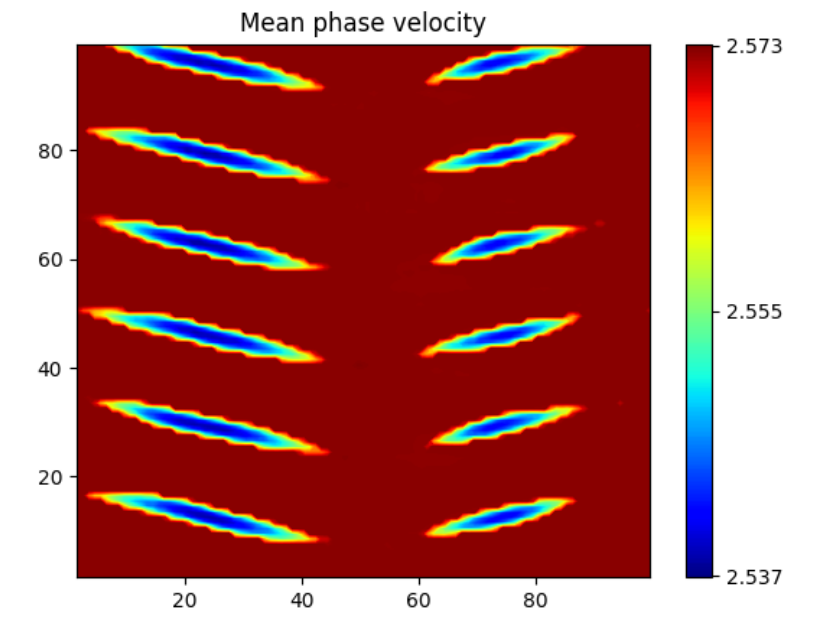
\includegraphics[width=0.8\textwidth]{Figures/mean_phase_velocity.png}
\caption{Double-Spotted Line}
\end{figure}

Με βάση τη θεωρητική ανάλυση των δύο σειριακών αλγορίθμων, το παλιό πρόγραμμα απαιτεί $N^2$ προσπελάσεις για τον υπολογισμό ενός δυναμικού, ενώ το νέο απαιτεί $(2R+1)^2$. Συνεπώς, με βάση τις παραμέτρους που αναφέρθηκαν, περιμένουμε πως το παλιό πρόγραμμα θα είναι $N^2/(2R+1)^2 \approx 5$ (τάξη μεγέθους) φορές πιο αργό. Στο Σχήμα 8 βλέπουμε τη συγκριτική απόδοση των δύο αλγορίθμων όπως εκτελέστηκαν στον υπολογιστή του εργαστηρίου.

\begin{figure}[h!]
\centering
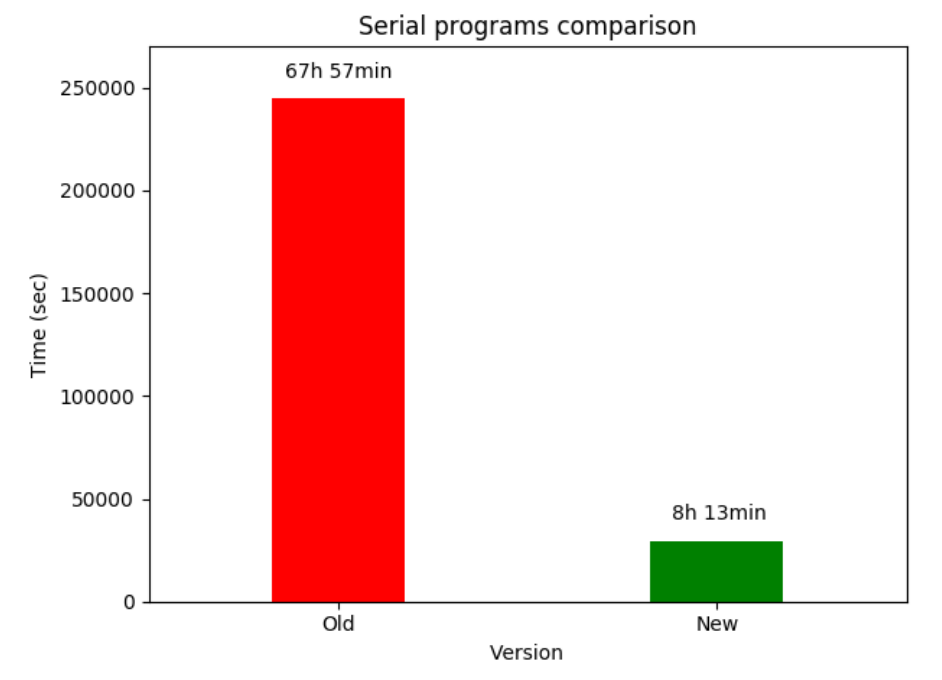
\includegraphics[width=0.8\textwidth]{Figures/oldvsnew.png}
\caption{Σύγκριση σειριακών προγραμμάτων}
\end{figure}
 
Πράγματι, μπορούμε να παρατηρήσουμε ότι το νέο πρόγραμμα είναι περίπου 8 φορές πιο γρήγορο. Η επιπλέον βελτίωση από τον αριθμό 5 που αναφέρθηκε προηγουμένως οφείλεται σε μικρές τροποποιήσεις που έχουν να κάνουν κυρίως με την περίοδο εφησυχασμού.

\subsection{Παραλληλοποίηση με PThreads και OpenMP}

Σε αυτή την ενότητα παρατηρούμε τη βελτίωση που παρουσιάζεται στη χρονική απόδοση του προγράμματος με τη χρήση των μεθόδων παραλληλοποίησης Pthreads και OpenMP που αναφέρθηκαν στα Κεφάλαια 2, 3.

Σε πρώτη φάση γίνεται σύγκριση των μεθόδων όπως εκτελέστηκαν στον υπολογιστή του εργαστηρίου με βάση τις παραμέτρους της προηγούμενης ενότητας. Η προσομοίωση πραγματοποιήθηκε και με τις δύο μεθόδους κάνοντας χρήση 2, 4 και 5 πυρήνων του επεξεργαστή. Τα αποτελέσματα παρουσιάζονται στο Σχήμα 9.

\begin{figure}[h!]
\centering
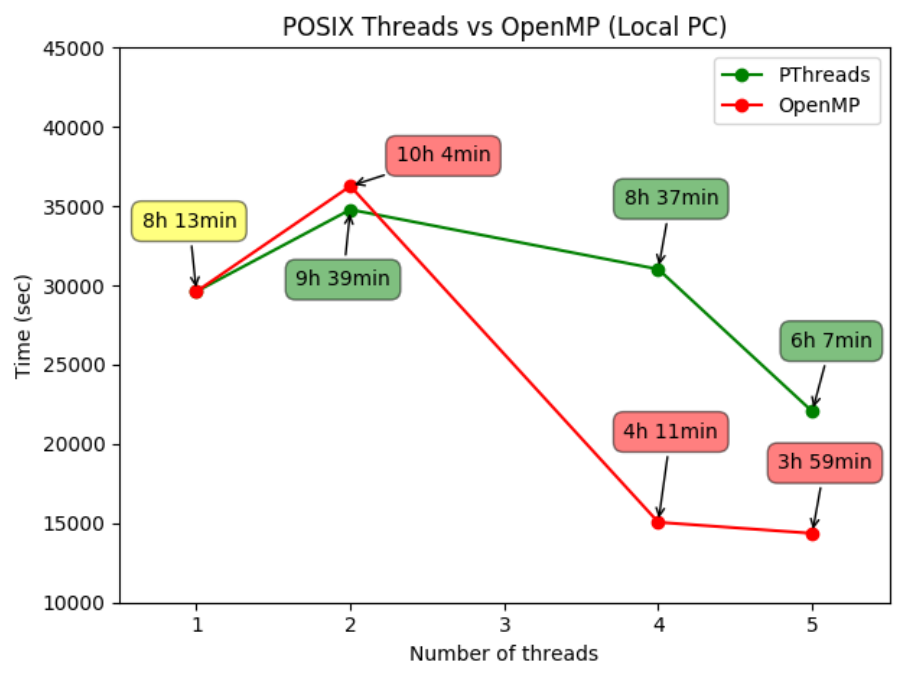
\includegraphics[width=0.8\textwidth]{Figures/posvsomp.png}
\caption{Σύγκριση PThreads με OpenMP (Τοπικά)}
\end{figure}

Είναι εύκολο να παρατηρήσουμε από το Σχήμα 9 ότι και στα δύο είδη παραλληλοποίησης, το πρόγραμμα παρουσιάζει μία αύξηση του χρόνου εκτέλεσης για μικρό αριθμό πυρήνων. Αυτό συμβαίνει επειδή η ύπαρξη πολλαπλών νημάτων απαιτεί διαδικασίες συγχρονισμού. Έτσι, παρόλο που κάθε νήμα εκτελεί ένα μικρότερο μέρος των υπολογισμών, ο επιπλέον χρόνος που προστίθεται ώστε τα νήματα να ενημερώσουν το ένα το άλλο για την εξέλιξη των εργασιών τους είναι σημαντικός. Για μεγαλύτερο αριθμό πυρήνων, βλέπουμε ότι τα προγράμματα όντως παρουσιάζουν βελτίωση σε σχέση με το σειριακό, κάτι που είναι αναμενόμενο, αφού οι υπολογισμοί για κάθε νήμα είναι αισθητά λιγότεροι όσο αυξάνονται οι διαθέσιμοι πυρήνες.

Η άλλη ενδιαφέρουσα παρατήρηση από το Σχήμα 9 είναι ότι το OpenMP παρουσιάζει καλύτερη χρονική απόδοση σε σχέση με το PThreads. Βασική αιτία για αυτή τη συμπεριφορά είναι η οδηγία \textit{schedule(dynamic)} που έχει δοθεί κατά την υλοποίηση του προγράμματος χρησιμοποιώντας το OpenMP. Σύμφωνα με αυτή την οδηγία, η ανάθεση των στοιχείων του πλέγματος στα νήματα γίνεται δυναμικά. Το χαρακτηριστικό του προγράμματος που κάνει αυτή την οδηγία χρήσιμη είναι το τμήμα του κώδικα που αφορά την περίοδο εφησυχασμού.

Αν το πρόγραμμα κρίνει ότι ένα στοιχείο βρίσκεται σε περίοδο εφησυχασμού, η ροή μπορεί να προχωρήσει στο επόμενο στοιχείο καθώς το δυναμικό θα παραμείνει μηδενικό και δεν υπάρχει λόγος να πραγματοποιηθούν υπολογισμοί. Λόγω του φαινομένου του συγχρονισμού και της ύπαρξης χιμαιρικών καταστάσεων, υπάρχουν σειρές του πλέγματος (συγχρονισμένες) που σε δεδομένες επαναλήψεις της προσομοίωσης όλα τα στοιχεία τους βρίσκονται σε περίοδο εφησυχασμού, ενώ άλλες σειρές (ασυγχρόνιστες) περιλαμβάνουν στοιχεία που απαιτούν υπολογισμό του δυναμικού τους. Σε αυτή την περίπτωση, στο πρόγραμμα με χρήση PThreads ορισμένα νήματα που αντιστοιχούν σε συγχρονισμένες γραμμές ολοκληρώνουν τη λειτουργία τους νωρίτερα από άλλα που αντιστοιχούν σε ασυγχρόνιστες οδηγώντας σε υποχρησιμοποίηση των διαθέσιμων πυρήνων. Αντιθέτως, στο πρόγραμμα που χρησιμοποιεί το OpenMP, αφού η ανάθεση γίνεται δυναμικά, οι ασυγχρόνιστες περιοχές και συνεπώς οι υπολογισμοί κατανέμονται ισόποσα ανάμεσα στους διαθέσιμους πυρήνες οδηγώντας σε καλύτερη εκμετάλλευση της υπολογιστικής ισχύος.

Προκειμένου να εξεταστεί περισσότερο οι σχέση των δύο προγραμματιστικών περιβαλλόντων εκτελέστηκαν προσομοιώσεις με ίδιες παραμέτρους και αρχικές συνθήκες και στον υπερυπολογιστή Άρη, όπου ο διαθέσιμος αριθμός πυρήνων είναι πολύ μεγαλύτερος. Αρχικά, παρουσιάζεται η διαφορά στη χρονική απόδοση μεταξύ του Άρη και του τοπικού υπολογιστή για μικρό αριθμό πυρήνων στο Σχήμα 10.

\begin{figure}[h!]
\centering
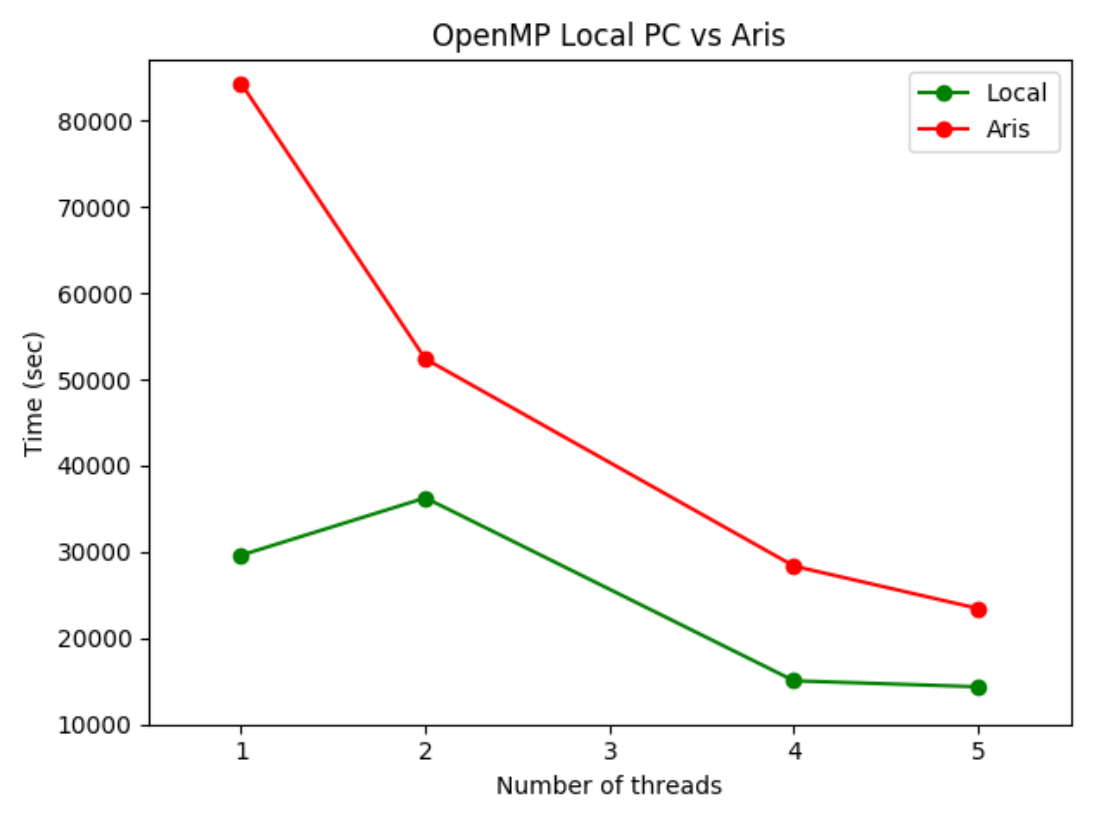
\includegraphics[width=0.8\textwidth]{Figures/localvsaris.png}
\caption{Σύγκριση τοπικού υπολογιστή με Άρη}
\end{figure}

Βλέπουμε πως η χρονική απόδοση είναι καλύτερη στο τοπικό μηχάνημα. Αυτό συμβαίνει επειδή υπερυπολογιστές όπως ο Άρης δίνουν βαρύτητα στην ύπαρξη πολύ μεγάλου αριθμού επεξεργαστών και όχι τόσο στην επιμέρους ταχύτητα των επεξεργαστών. Μία σημαντική παρατήρηση είναι πως η αύξηση στο χρόνο εκτέλεσης από 1 σε 2 πυρήνες που παρατηρείται στο τοπικό μηχάνημα δεν συμβαίνει στον Άρη. Ο λόγος για αυτή τη διαφοροποίηση είναι ότι ο υπερυπολογιστής είναι βελτιστοποιημένος ώστε να είναι ελάχιστα τα context switch που συμβαίνουν και η επιβάρυνση που προσθέτει ο παραλληλισμός να μην είναι τόσο σημαντική. Για 4 και 5 πυρήνες, η διαφορά μεταξύ των δύο γραφημάτων μειώνεται αισθητά, κάτι που είναι αναμενόμενο αφού η καθυστέρηση του Άρη για το σειριακό πρόγραμμα μοιράζεται ισόποσα στους πολλαπλούς επεξεργαστές.

Στη συνέχεια, οι δύο μέθοδοι δοκιμάστηκαν κάνοντας χρήση 2, 4, 5, 10, 20, 25 και 50 πυρήνων του υπερυπολογιστή. Τα αποτελέσματα των προσομοιώσεων φαίνονται στο Σχήμα 11.

\begin{figure}[h!]
\centering
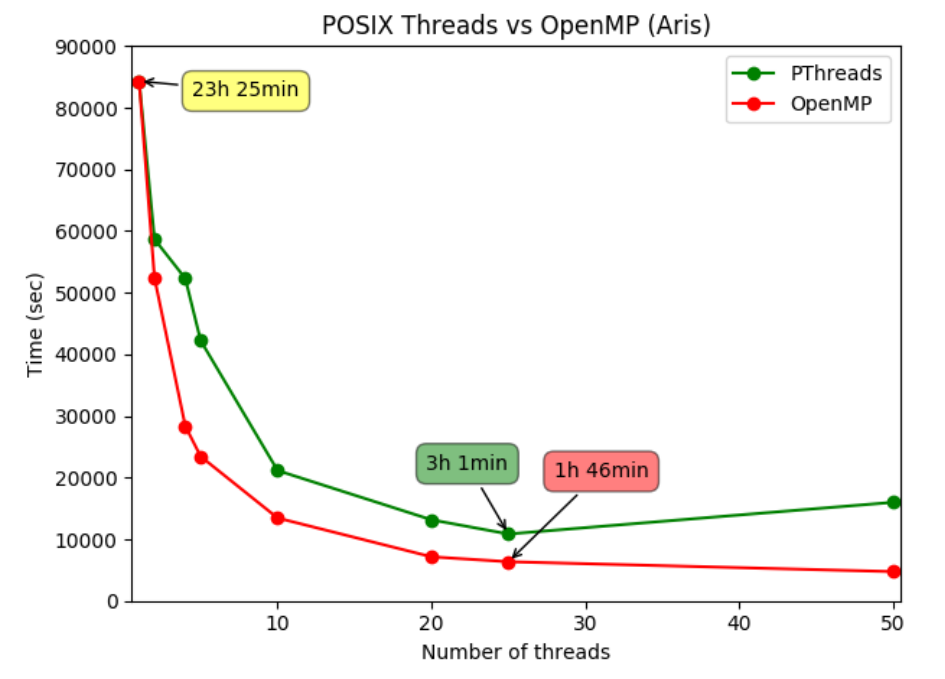
\includegraphics[width=0.8\textwidth]{Figures/arisposvsomp.png}
\caption{Σύγκριση PThreads με OpenMP (Άρης)}
\end{figure}

Από το Σχήμα 11 μπορούμε εύκολα να δούμε ότι ό χρόνος εκτέλεσης μειώνεται σε πολύ μεγάλο βαθμό χρησιμοποιώντας μεγάλο αριθμό πυρήνων, κάτι που ήταν αναμενόμενο από την αρχή λόγω της φύσης του προβλήματος και των δυνατοτήτων παραλληλοποίησης που προσφέρει.

Μία παρατήρηση που αξίζει να αναφερθεί είναι ότι τα δύο προγράμματα παρουσιάζουν την ίδια συμπεριφορά ως προς την απόδοση όσο μεταβάλλεται ο βαθμός παραλληλισμού. Φαίνεται και τα δύο να παρουσιάζουν κάποιο κάτω φράγμα το οποίο προσεγγίζεται όσο ο αριθμός των πυρήνων αυξάνεται. Η διαφορά των δύο γραφικών παραστάσεων οφείλεται στα χαρακτηριστικά του OpenMP που αναφέρθηκαν προηγουμένως και αγγίζει τη διαφορά περίπου μιας ώρας.

Με βάση τα παραπάνω στοιχεία, μπορούμε να καταλήξουμε με ασφάλεια ότι το προγραμματιστικό περιβάλλον που παρουσιάζει την καλύτερη απόδοση είναι το OpenMP. Γι' αυτό το λόγο, πραγματοποιήθηκαν περαιτέρω δοκιμές με ενδιάμεσο αριθμό πυρήνων, ώστε να υπάρχει μια πιο ακριβής απεικόνιση της απόδοσης σε σχέση με το βαθμό παραλληλισμού. Τα αποτελέσματα φαίνονται στο Σχήμα 12.

\begin{figure}[h!]
\centering
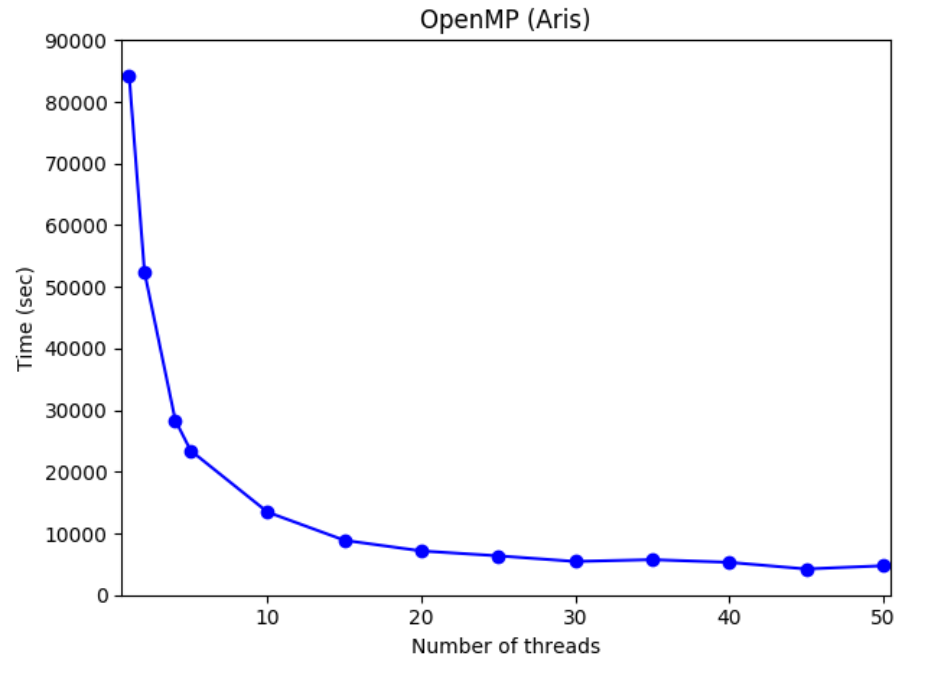
\includegraphics[width=0.8\textwidth]{Figures/omp.png}
\caption{Αναλυτική συμπεριφορά OpenMP (Άρης)}
\end{figure}  

Μπορούμε να δούμε ότι η γραφική παράσταση αρχικά είναι γραμμική, δηλαδή η απόδοση είναι αντιστρόφως ανάλογη του αριθμού πυρήνων. Κάτι τέτοιο παύει να ισχύει όσο ο αριθμός αυτός μεγαλώνει. Το κάτω φράγμα που παρουσιάζεται στην απόδοση οφείλεται στο αυξανόμενο ``κόστος'' των αναγκών συγχρονισμού μεταξύ των παράλληλων νημάτων. Όσο ο αριθμός των νημάτων που εκτελούν υπολογισμούς αυξάνεται, τόσο περισσότερος χρόνος απαιτείται για τη δημιουργία και την αναμονή τερματισμού τους. Αυτός ο επιπρόσθετος χρόνος λειτουργεί ως αντίβαρο στο ``κέρδος'' του παραλληλισμού.

\subsection{Παραλληλοποίηση με CUDA και Συνολικά Αποτελέσματα}

Σε αυτή την ενότητα παρουσιάζονται τα αποτελέσματα της τελευταίας μεθόδου παραλληλοποίησης με χρήση του προγραμματιστικού περιβάλλοντος CUDA και σε σύγκριση με τα αποτελέσματα των υπολοίπων μεθόδων.

Κάνοντας χρήση των υπολογιστικών δυνατοτήτων της κάρτας γραφικών, αναμένουμε πως η απόδοση του προγράμματος θα είναι πολύ καλύτερη από όλες τις προηγούμενες μεθόδους. Αυτό συμβαίνει διότι η κάρτα γραφικών περιέχει πολύ μεγαλύτερο αριθμό υπολογιστικών πυρήνων και από τον επεξεργαστή του τοπικού υπολογιστή και από τον υπερυπολογιστή Άρη. Συγκεκριμένα, η GPU που χρησιμοποιήθηκε περιέχει 1664 πυρήνες με επιπλέον δυνατότητα υποστήριξης πολλαπλών νημάτων ανά πυρήνα.

Για την υλοποίηση του προγράμματος με χρήση CUDA, έγινε μια απλή επιλογή για το διαμοιρασμό των εργασιών σε 100 Blocks με 100 Threads ανά Block. Τα αποτελέσματα με χρήση CUDA καθώς και κάποια από τα αποτελέσματα των προηγούμενων ενοτήτων φαίνονται στο παρακάτω συγκριτικό διάγραμμα.

\begin{figure}[H]
\centering
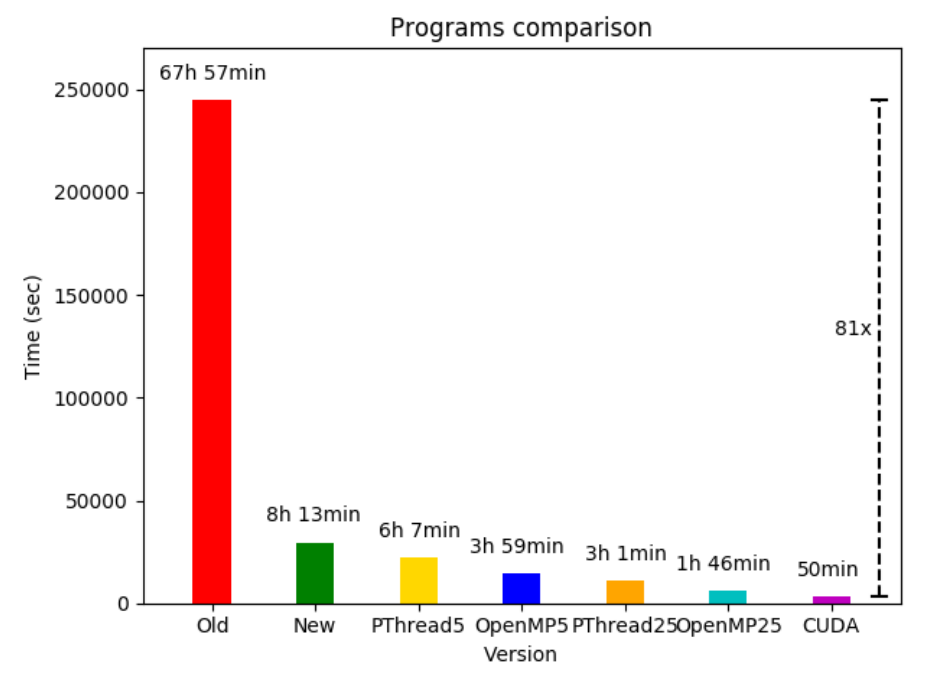
\includegraphics[width=0.8\textwidth]{Figures/total.png}
\caption{Απόδοση προγράμματος σε διαφορετικά προγραμματιστικά περιβάλλοντα}
\end{figure}  

\newpage

\section{Συμπεράσματα}

\subsection{Θετικά αποτελέσματα}

Από τα αποτελέσματα του Κεφαλαίου 4 μπορούμε εύκολα να συμπεράνουμε ότι οι μέθοδοι παραλληλοποίησης για την προσομοίωση βιολογικών νευρώνων είναι πλήρως απαραίτητες προκειμένου να εξαχθούν γρήγορα συμπεράσματα που αφορούν την εμφάνιση χιμαιρικών καταστάσεων. Η φύση του προβλήματος είναι κατάλληλη ώστε να μπορούν να πραγματοποιηθούν πολλαπλοί παράλληλοι υπολογισμοί ταυτόχρονα χωρίς να εξαρτώνται ο ένας από τον άλλο. Το αποτέλεσμα είναι μία πολύ μεγάλη αύξηση στην απόδοση του προγράμματος προσομοίωσης.

Όσον αφορά τις μεθόδους που χρησιμοποιήθηκαν, η μέθοδος που συνδυάζει τα καλύτερα χαρακτηριστικά ευκολίας υλοποίησης και χρονικής απόδοσης είναι η χρήση του προγραμματιστικού περιβάλλοντος OpenMP. Το μεγάλο πλεονέκτημα της μεθόδου είναι ότι απλοποιεί αρκετά τη διαδικασία παραλληλισμού για τον προγραμματιστή χωρίς να απαιτεί πλήρη έλεγχο των τεχνικών λεπτομερειών σε χαμηλό επίπεδο. Επίσης, από τις δοκιμές φάνηκε ότι το OpenMP δίνει πολύ ικανοποιητικά αποτελέσματα όταν εκτελείται σε μεγάλο αριθμό πυρήνων, κάνοντας χρήση των δυνατοτήτων κάποιου υπερυπολογιστή.

Βλέποντας αυστηρά το κομμάτι της χρονικής απόδοσης, το καλύτερο προγραμματιστικό περιβάλλον είναι το CUDA. Η χρήση του συνίσταται για παρόμοιους υπολογισμούς και είναι ένα πάρα πολύ χρήσιμο εργαλείο. Παρ' όλα αυτά, έχει το μειονέκτημα ότι η χρήση του χρειάζεται εξειδικευμένη γνώση των τεχνικών λεπτομερειών της λειτουργίας της κάρτας γραφικών. Επίσης, η διάθεση των απαιτούμενων υπολογιστικών πόρων (GPU) είναι αρκετά ακριβότερη και συνεπώς πιο σπάνια απ' ότι οι κλασικές μονάδες επεξεργασίας.

\subsection{Εμπόδια}

Το μεγαλύτερο εμπόδιο που παρατηρήθηκε είναι η δυσκολία βελτιστοποίησης του προγράμματος με χρήση PThreads. Το συγκεκριμένο εργαλείο δίνει πλήρη έλεγχο στον προγραμματιστή και συνεπώς έχει μεγαλύτερες δυνατότητες από το OpenMP, όπου και τα δύο υλοποιούν το μοντέλο παραλληλισμού νημάτων. Παρ' όλα αυτά, λόγω της δυσκολίας στην υλοποίηση, η αφιέρωση χρόνου για βελτιστοποίηση της χρήσης του συγκεκριμένου εργαλείου ενδεχομένως να μην αξίζει, δεδομένου ότι η χρήση του OpenMP με απλές παραμέτρους μπορεί να δώσει καλύτερα χρονικά αποτελέσματα.

\subsection{Ανοικτά προβλήματα}

Το πρόγραμμα με όλες του τις εκδοχές όπως περιγράφηκε στα πρώτα Κεφάλαια, σχεδιάστηκε προκειμένου να προσομοιώνει το μοντέλο νευρώνων Leaky Integrate-and-Fire πάνω σε δισδιάστατο πλέγμα με Μη-Τοπική Συνδεσιμότητα. Προκειμένου να γίνει χρήσιμο για ευρεία χρήση σε μελέτη φαινομένων χιμαιρικών καταστάσεων θα πρέπει να τροποποιηθεί ώστε να υποστηρίζει διαφορετικά μοντέλα διαφορικών εξισώσεων, πιο περίπλοκες τοπολογίες (π.χ. διαγώνια, φρακταλική) \cite{tsigkri-desmedt_multi-leveled_nodate} και περισσότερες διαστάσεις. Επίσης, έχει ενδιαφέρον το πώς τέτοιες αλλαγές θα επιδράσουν στη χρονική απόδοση του προγράμματος και σε ποιο βαθμό διατηρείται το ``κέρδος'' της παραλληλοποίησης.

Επίσης, ένα άλλο ερώτημα τεχνικής φύσεως είναι το κατά πόσο μπορεί να βελτιωθεί περαιτέρω η χρονική απόδοση του προγράμματος στο προγραμματιστικό περιβάλλον CUDA. Για την πραγματοποίηση των προσομοιώσεων χρησιμοποιήθηκε ένας απλός διαμοιρασμός των υπολογισμών σε 100 Blocks με 100 Threads ανά Block. Είναι αυτός ο διαμοιρασμός βέλτιστος ή υπάρχει κάποια πιο ειδική στρατηγική που να εκμεταλλεύεται τα χαρακτηριστικά του hardware προκειμένου να βελτιστοποιεί την απόδοση;

Επίσης, ως τελευταίο στάδιο, θα είχε ενδιαφέρον η εκτέλεση του προγράμματος σε CUDA, στον υπερυπολογιστή Άρη κάνοντας χρήση κόμβων με πολλαπλές GPU. Έτσι, θα μπορούσε να γίνει ταυτόχρονη προσομοίωση πολλαπλών αρχικών συνθηκών, κάτι που είναι αδύνατο στον υπολογιστή του εργαστηρίου αφού διατίθεται μία GPU. Επίσης, θα μπορούσε να εξεταστεί το ενδεχόμενο να εκτελεστεί ένα μοναδικό στιγμιότυπο του προγράμματος μοιράζοντας τους υπολογισμούς σε πάνω από μία GPU, επιταχύνοντας ακόμη περισσότερο τη χρονική απόδοση, κάτι που θα ήταν ιδιαίτερα χρήσιμο αν το μέγεθος του συστήματος υπό μελέτη ήταν μεγαλύτερο (π.χ. $1000 \times 1000$).

\newpage

\bibliographystyle{unsrt}
\bibliography{internship}
\newpage

\appendix
\section{Παράρτημα}

Εδώ παρατίθεται ο κώδικας που εκτελεί την προσομοίωση κάνοντας τη χρήση του εργαλείου OpenMP. Για την εκτέλεση του σειριακού προγράμματος χωρίς παραλληλοποίηση, αρκεί η αφαίρεση των δύο γραμμών που αρχίζουν με την οδηγία \#pragma.

\lstinputlisting[language=C,frame=single]{Code/LIF_2D_Classic_OpenMP.c}

\end{document}